\chapter{Projektmonitoring}
\label{projektmonitoring}

\section{Projektverlauf}
In Abbildung \ref{overall_stories_gantt_chart} sind alle erledigten Stories mit Start- und Endpunkt auf der Zeitachse abgebildet. Leider werden die Sprints etwas verfälscht dargestellt, da wir einzelne bereits begonnene Stories aus Zeitgründen von einem Sprint in den nächsten verschoben haben (Stories \#25, \#113 und \#186). Diese werden von Redmine dann über mehrere Sprints hinweg dargestellt, was natürlich auch den Sprint künstlich "`verlängert"'.

\begin{figure}[H]
	\centering
	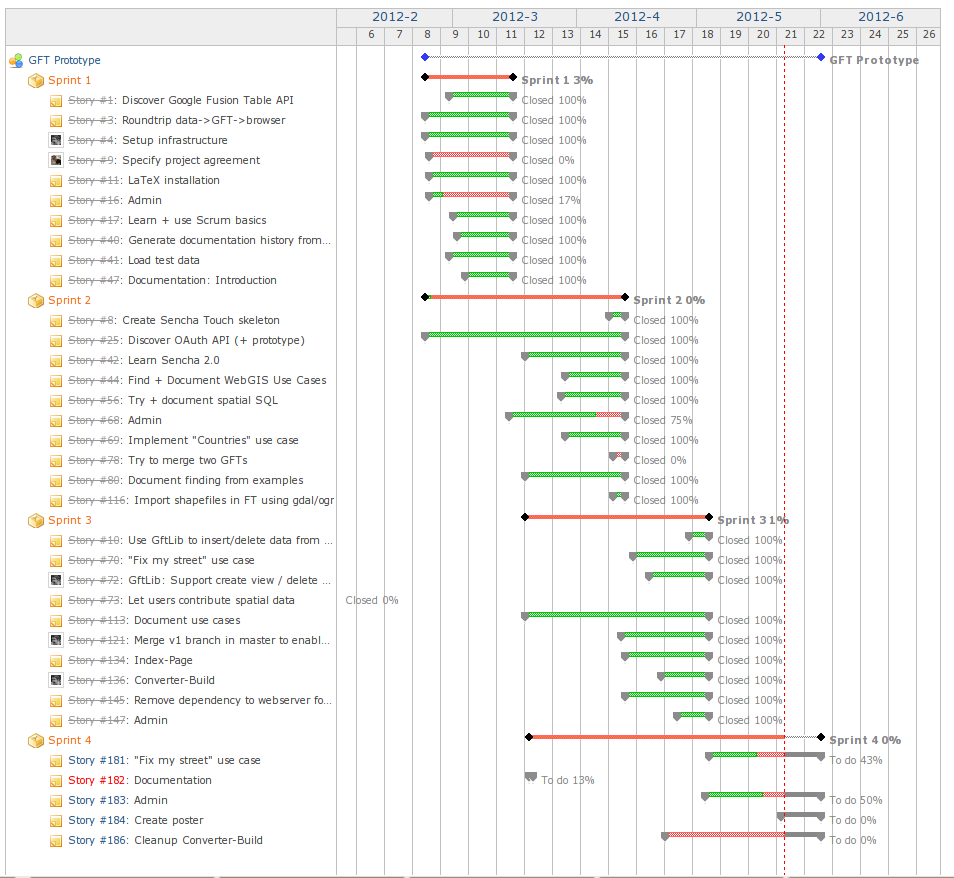
\includegraphics[width=\textwidth]{images/projektmanagement/overall_stories_gantt_chart}
	\caption{Gantt-Diagramm des Projektverlaufs}
	\label{overall_stories_gantt_chart}
\end{figure}

\section{Arbeitsaufwand}
Wie schon im Kapitel \ref{projektmanagement} beschrieben, war der vom Modul vorgegebene Aufwand pro Person auf \emph{240 Stunden} festgelegt. Wie in der Tabelle \ref{projektmanagement-arbeitsaufwand} ersichtlich haben wir diese Vorgabe beide leicht überschritten.

\begin{longtable}{|l|l|}
\hline 
\textbf{Person} & \textbf{Aufwand} \\ 
\hline 
Stefan Oderbolz & 250h \\ 
\hline 
Jürg Hunziker & 260h \\ 
\hline 
\caption{Arbeitsaufwand pro Person}
\label{projektmanagement-arbeitsaufwand}
\end{longtable} 

\section{Fazit}
\todo[inline]{Projektverlauf Fazit schreiben}